% Author: Izaak Neutelings (June, 2018)
\documentclass[border=3pt,tikz]{standalone}
\usepackage{ifthen}
\usepackage{siunitx}
\usepackage{tikz}
\usetikzlibrary{hobby} % for ..
\usetikzlibrary{arrows.meta} % to control arrow size
\usetikzlibrary{decorations.text}
\tikzset{>={Latex[length=4,width=4]}} % for LaTeX arrow head
\usetikzlibrary{calc,intersections,decorations.markings}
\usepackage{siunitx}
\usepackage{xcolor} % for colored text

\colorlet{mylightblue}{blue!20}
\colorlet{myblue}{blue!50!black}
\colorlet{mydarkblue}{blue!30!black}
\colorlet{mylightred}{red!10}
\colorlet{myred}{red!50!black}
\colorlet{mydarkred}{red!60!black}
\colorlet{mydarkgreen}{green!30!black}

%\tikzstyle{midarr}=[decoration={markings,mark=at position 0.5 with {\arrow{stealth}}},postaction={decorate}]
\tikzset{
    midarr/.style={decoration={markings,mark=at position #1 with {\arrow{stealth}}},postaction={decorate}},
    midarr/.default=0.5
}
\def\tick#1#2{\draw[thick] (#1) ++ (#2:0.03*\ymax) --++ (#2-180:0.06*\ymax)}


\begin{document}

% PHASE DIAGRAM
    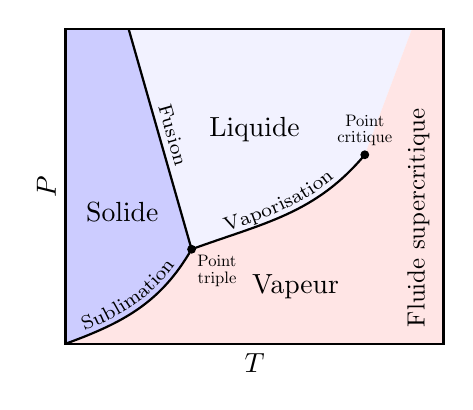
\begin{tikzpicture}[scale=0.4]
        \message{Phase diagrams^^J}

        \def\xtick#1#2{\draw[thick] (#1)++(0,.2) --++ (0,-.4) node[below=-.5pt,scale=0.7] {#2};}
        \def\ytick#1#2{\draw[thick] (#1)++(.2,0) --++ (-.4,0) node[left=-.5pt,scale=0.7] {#2};}

        % COORDINATES
        \coordinate (O) at (0,0);
        \coordinate (N1) at (2,10);
        \coordinate (N2) at (11,10);
        \coordinate (NE) at (12,10);
        \coordinate (NW) at (0,10);
        \coordinate (SE) at (12,0);
        \coordinate (W) at (0,5);
        \coordinate (S) at (6,0);
        \coordinate (C) at (9.5,6); % critical
        \coordinate (T) at (4,3); % triple

        % PATHS
        \def\SL{(T) -- (N1)}
        \def\SG{(O) to[out=20,in=-120] (T)}
        \def\LG{(T) to[out=20,in=-130] (C)}
        \def\atm{(0,5.5) -- (12,5.5)}
        \path[name path=LG] \LG;
        \path[name path=atm] \atm;

        % REGIONS
        \fill[mylightblue] \SG -- (N1) -- (NW) -- cycle;
        \fill[blue!5] \LG -- (N2) -- (N1) -- cycle;
        \fill[mylightred] \LG -- (N2) -- (NE) -- (SE) -- \SG -- cycle;
        \node at (1.8,4.2) {Solide};
        \node at (7.3,1.8) {Vapeur};
        \node at (6,6.8) {Liquide};

        \node [rotate=90,scale=0.9] at (11.2,4) {Fluide supercritique};

        % POINTS
        \fill (T) circle (4pt) node[below right,scale=0.6,align=right] {Point\\[-2pt]triple};
        \fill (C) circle (4pt) node[above=1pt,scale=0.6,align=center] {Point\\[-2pt]critique};

        % LINES
        \def\lineLegend#1{\scriptsize\raisebox{2pt}}

        \draw[thick,postaction={decorate,decoration={text along path,text align=center,text={|\lineLegend|Sublimation}}}] \SG;
        \draw[thick,postaction={decorate,decoration={text along path,text align=center,text={|\lineLegend|Vaporisation}}}] \LG;
        \draw[thick] \SL;
        \draw \SL node[midway, above=-1pt, sloped] (TextNode) {\scriptsize Fusion};

        % AXES
        \draw[thick] (O) rectangle (NE);
        \node[left=0pt,above,rotate=90] at (W) {$P$};
        \node[below=0pt] at (S) {$T$};

    \end{tikzpicture}

\end{document}
